

\subsection{Applying Kernel PCA}

\begin{frame}{How do I interpret the role of PCs?}

\notesonly{\question{How do I interpret the role of PCs?}}

\svspace{-7mm}

\begin{center}
	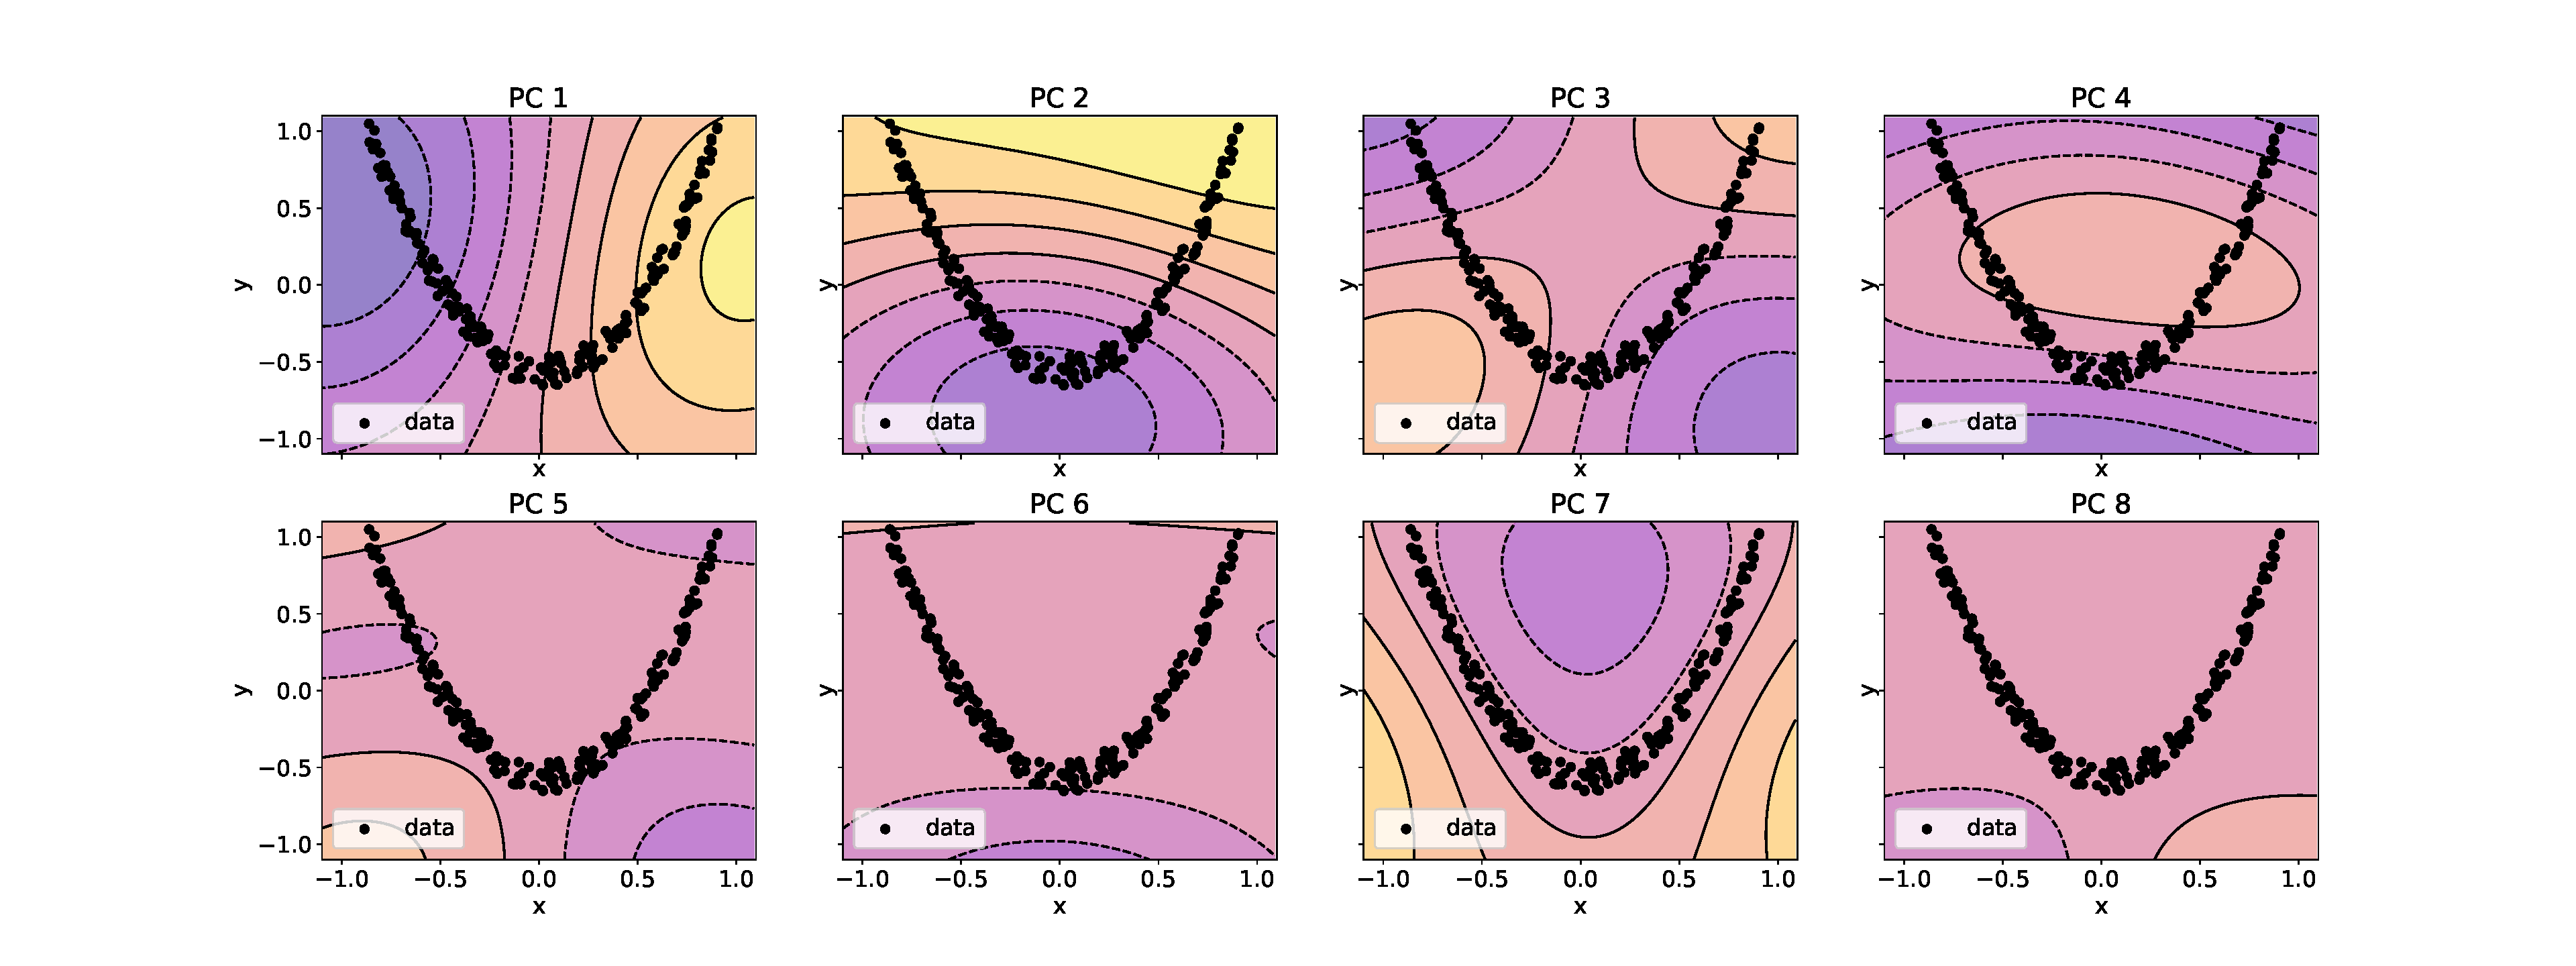
\includegraphics[height=5cm]{img/contourplot_kpca_rbf}
	\notesonly{\captionof{figure}{Projections onto individual PCs}}
\end{center}
\svspace{-0.8cm}
\begin{center}
	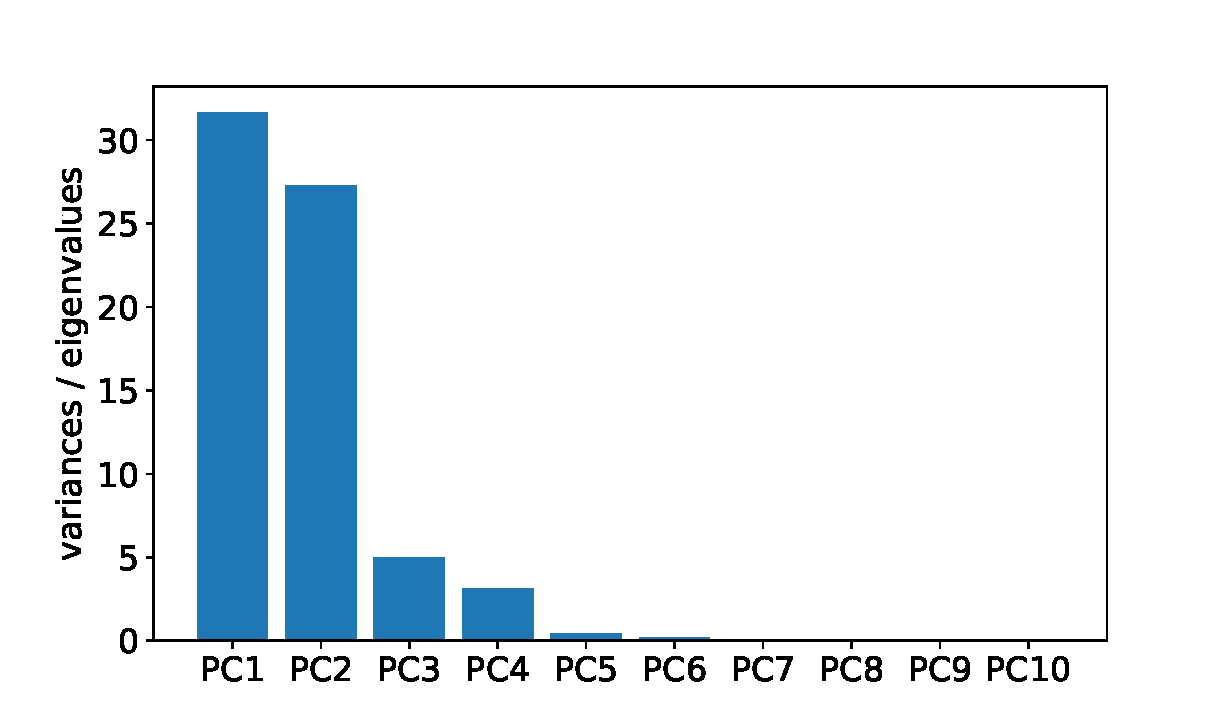
\includegraphics[height=3.2cm]{img/screeplot_kpca_rbf.pdf}
	\notesonly{\captionof{figure}{Scree plot}}
\end{center}

\end{frame}

\subsection{A note on implementation}

\begin{frame}{\subsecname}

\question{Should you solve the transformed eigenvalue problem using \emph{eigenvalue decomposition} or \emph{SVD}?}

\slidesonly{
\begin{equation}
%\label{eq:eigsimple1}
	\vec{K} \, \vec{a} = p \lambda \vec{a}
\end{equation}
}

\pause

- \emph{eigenvalue decomposition} is the only option for Kernel PCA. \emph{SVD} is simply not applicable since we don't have access to $\vec \phi_{((\vec x))}$

\begin{equation}
 %\label{eq:cov}
\vec C_{\phi} = \frac{1}{p} \sum_{\alpha=1}^{p} \vec{\phi}_{(\vec{x}^{(\alpha)})} \vec{\phi}^{\top}_{(\vec{x}^{(\alpha)})}
\end{equation}

\end{frame}

\begin{frame}{\subsecname}

\question{Which property of $\widetilde {\vec{K}}$ can we exploit to speed up computation?}

\pause

The kernel function is symmetric. $k(\vec x^{(\alpha)}, \vec x^{(\beta)}) = k(\vec x^{(\beta)}, \vec x^{(\alpha)})$. One can exploit this by reducing how many times the kernel function is actually applied while traversing the training samples when computing $\widetilde {\vec{K}}$.

\end{frame}

%TL;DR: Picking the right parameters for the kernel depends on how good that parameter solves your problem (good dim. reduction, reflects certain assumptions about the data - e.g. expected degree of polynomial). We treat them as hyperparameters, so "tuning" them is usually done through cross-validation than gradient-based optimization.

%The long version. This is actually how I end up with more content for the tutorial notes, not always but every now and then it happens. So thank you for the question:

%Finding good parameters for the kernels depends on the data and the task you are trying to solve.
%This comes across as a very generic answer but let's look at two examples. I will use the RBF Kernel which is parameterized by a single parameter sigma. You an easily extend this to other kernels. It also doesn't matter if we're using this kernel for an unsupervised method (e.g. Kernel PCA) or a supervised one (e.g. SVM - don't feel left out if you don't know what an SVM is - just don't tell anyone - people are so judgmental these days tsts):

%Example A: We want to reduce the dimensionality of some high dimensional data (i.e. compression). We start of with N dimensions (N is large), p points (lots of points). Kernel PCA is going to give us p PCs. We perform Kernel PCA once with sigma = sigma_1 and a second time with sigma = sigma_2.
%How do we know which sigma value to use for dimensionality reduction?

%Suggestion 1: Create a scree plot for the eigenvalues obtained from using sigma_1 and compare it to the scree plot from using sigma_2. The ones that gives you "more variance explained" with the least amount of PCs is an indication that one sigma could be better than the other. A scree plot that shows a lot of variance explained for the first couple of PCs and then suddenly drops for all the rest is an indicator that those PCs are enough for good dimensionality reduction. You'll sometimes run into situations where you don't think the comparison shows a clear winner. Therefore,...

%Suggestion 2: Measure and compare reconstruction error between the two sigmas. It's exactly what we're looking for when doing dimensionality reduction. More intuitive than looking at a scree plot but it involves reconstructing and that involves approximations (c.f. lecture slide 1.4 #23) so there's a drawback.
%Something to keep in mind when using reconstruction error is that for the same sigma you get some value for your reconstruction error when measure it for data that you used in training (i.e. solving the eigenvalue problem) vs. the error value you get when reconstructing test data. This is where cross validation comes in. We're going to talk about cross-validation later in the course when we talk about density estimation. Basically, you want to know how well your model does when you feed it data that it's never seen before. If it does well on training data but badly on unseen data, then you can't really deploy this model. So before deploying it you need to measure this performance (e.g. reconstruction error) on unseen data. This is called cross validation and you can use this to compare how well one sigma does vs another. How well does one sigma do on unseen data vs. the other sigma? The sigma that has better cross validation performance is the one you go with.

%Example B: Using Kernel PCA to preprocess data before feeding it into a classifier:
%You've picked a kernel (e.g. RBF) you're trying different values for the sigma. You do Kernel PCA and project the data onto the PCs. You feed the projections into a classifier to tell you if this is an image of a cat or a dog (TODO: cat vs. dog is boring, replace with something that has more bling). You measure the classifier's performance and you find out it gives the correct answer 80% of the time. Redo the above with another sigma and you get 87%. You can use the classifier's performance as a measure for deciding which sigma to use. It's still Kernel PCA but you're hyperparameter selection is based on something completely different. But it's a well justified criterion for that task that you are trying to solve. Calling a parameter a "hyperparameter" implies that you don't used gradient-based optimization to tune it but rather something like cross-validation. The reason for not using gradient-based optimization could be that you performance measure or cost function w.r.t. to that parameter is not necessarily differntiable or it would make the optimization too complicated from all the free parameters.

%A note on the Neural Network kernel (aka tanh Kernel, aka sigmoid kernel):
%The kernel itself is not a neural network. when people saw the expression tanh( xTx + ) resembled an expression we are used to seeing in neural networks. What value do you pick for and ? Scroll up, the same applies and it depends on the data and the task.
